
\subsection{Medición de Parámetros de un Amplificador}

Muchos circuitos electrónicos se pueden representar como cuadripolos con parámetros concentrados. En el caso de los amplificadores, para simplificar su análisis numérico y de comportamiento, se los puede representar como un cuadripolo constituido por: una impedancia de entrada $Z_i$ (en paralelo con la fuente de señal de entrada $v_i$); una fuente de tensión $v_o$, con un valor de tensión igual al de la entrada multiplicada por un factor (Ganancia $A$); y en serie con esta fuente interna, una impedancia de salida $Z_o$. Este modelo se puede apreciar en la figura \ref{fig:cuadAmp}

\begin{figure}[h]
    \centering
    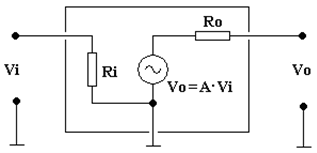
\includegraphics[width=0.45\linewidth]{Imagenes/cuadAmp.png}
    \caption{Circuito equivalente de una amplificador genérico}
    \label{fig:cuadAmp}
\end{figure}

La forma de medir cada uno de estos parámetros se presentará a continuación.

Cabe destacar, que los métodos revelados a continuación aplican principalmente para circuitos amplificadores de señales de bajas frecuencias, donde la contribución de los fenómenos reactivos (tanto capacitivos como inductivos) es despreciable.

\subsubsection{Impedancia de Entrada}
\label{sec:Zi}

La forma más directa de medir la impedancia de entrada de un amplificador, teniendo en cuenta la consideración previamente anunciada, es mediante el uso de una resistencia variable en serie, entre la fuente de señal y el amplificador.

Primero y antes de conectar esa resistencia, será necesario medir la tensión de salida $v_o$ para la señal de máxima amplitud que el amplificador pueda soportar, sin entrar en zona de funcionamiento alineal (recortar alguno de los picos). Esto se realiza exclusivamente con la finalidad de lograr trabajar con señales más grande para que así sea mas fácil analizarlas y que se vean menos afectadas por el ruido. Una vez obtenido este valor, se procede a conectar la resistencia variable y se lleva la tensión de salida a la mitad del valor medido anteriormente. 

Al poner la resistencia variable de prueba en serie con la $Z_i$, se está creando un divisor resistivo. Y se sabe que cuando un divisor resistivo esta compuesto de dos resistencias de igual valor, la tensión que cae en la segunda resistencia, es la mitad de la tensión de entrada. 

Por lo que si aquí se tiene la mitad de la señal de salida, con una ganancia constante, lo que se modificó fue la tensión de entrada $v_i$ (del cuadripolo, no del generador), la cual también fue llevada a la mitad de su valor original.

Conectando los puntos, se ve que para que la señal de entrada sea de la mitad de su valor original, las resistencias del divisor deben tener el mismo valor. Por lo que el resistor variable ahora es del mismo valor que la impedancia/resistencia de entrada $Z_i$.

Para medir este valor, se desconecta la resistencia variable y se mide con un óhmetro con la mayor exactitud posible.

\subsubsection{Impedancia de Salida}
\label{sec:Zo}

Para la impedancia de salida, se aplica el mismo concepto que para la de entrada, salvo que en este caso la resistencia variable de prueba irá a la salida del cuadripolo. 

Partiendo de la tensión de salida de máxima amplitud, se conecta la resistencia de prueba y se modifica su valor hasta que este sea la mitad del valor original. Una vez en este punto, se retira la resistencia y se mide con un óhmetro su valor. Este será el valore de la impedancia/resistencia de salida $Z_o$.

Una alternativa al uso de resistencias variables, pero donde también se emplea el concepto de divisor resistivo, es el que se ve en la figura \ref{fig:medRo}.

\begin{figure}[h]
    \centering
    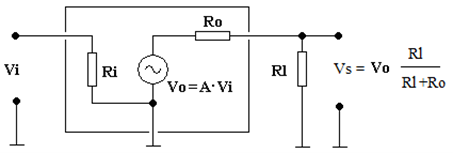
\includegraphics[width=0.6\linewidth]{Imagenes/medRo.png}
    \caption{Esquema de medición de $R_o$}
    \label{fig:medRo}
\end{figure}

El esquema de conexión es igual que el anterior, pero ahora se utilizará una resistencia de valor conocido y constante. Se plantea la ecuación de la tensión $v_s$ de salida de la figura en base a $v_o$ (tensión de salida del cuadripolo). A partir de esta se despeja $R_o$ (ecuación \ref{eq:Ro}) y ya se puede calcular la impedancia de salida del amplificador en base a la tensión de salida en vacío $v_o$, la tensión de salida con la carga $v_s$ y la resistencia de carga $R_l$.

\begin{equation}
    v_s = v_o \cdot \cfrac{R_l}{R_l + R_o}
    \hspace{5mm}\Longrightarrow\hspace{5mm}
    R_o = R_l \cdot \left( \cfrac{v_o}{v_s} - 1 \right)
    \label{eq:Ro}
\end{equation}

Estos métodos de medición, son útiles solamente para amplificadores no realimentados. Cuando se conecta el lazo de realimentación, puede haber dificultades porque uno de los efectos de la realimentación es mantener estable la amplitud de la salida del amplificador, aunque varíe la carga conectada, lo cual implica una reducción de la resistencia de salida.
Si se intenta variar la carga hasta que la tensión de salida se reduzca a la mitad de la que hay sin carga, puede ocurrir que se lleve el punto de funcionamiento del amplificador a una zona donde la potencia disipada exceda los limites previstos y se dañe.


\subsubsection{Ganancia}\label{sec:Gan}


La ganancia $A$ de un amplificador, tanto a lazo abierto como a lazo cerrado, se pude medir fácilmente midiendo la tensión de entrada $v_i$ y la tensión de salida $v_o$, y luego calculando la relación entre ambas (ecuación \ref{eq:ganancia}).

\begin{equation}
    A = \cfrac{v_o}{v_i}
    \label{eq:ganancia}
\end{equation}

Se debe tener en cuenta que la tensión de salida $v_o$ es a bornes de la fuente interna del cuadripolo, o a bornes de este, cuando está en vacío (sin carga).  

Además de este, existen otros métodos para calcular la ganancia a partir de la potencia, los cuales se verán en la próxima sub-sección.



\vspace{1.5cm}
\subsection{Medición de potencia con instrumentos calibrados en decibelios}

El decibelio o $\mathrm{dB}$ es una unidad muy útil cuando se intenta medir relaciones o razones entre una salida y una entrada. Es aún más útil cuando se intenta medir algún valor como la ganancia de potencia en amplificadores, teniendo en cuenta que un amplificador puede contar con varias etapas, y su ganancia puede ser un valor muy elevado. El decibelio permite expresar esta relación de gran valor en una escala logarítmica más legible para el análisis.

\begin{equation}
    P_{dB} = 10\cdot\log{\frac{P_o}{P_i}}
\end{equation}

En cierto modo, el decibelio se utiliza para medir cuanto se "aleja" un valor de su referencia inicial (entrada). Si el valor de entrada no está especificado o no existe, por lo general, la referencia es la unidad, pero cuando se realiza cálculos de potencia, resulta útil utilizar otras referencias. Una de ellas es la referencia a 1mW, y cuando la medición en decibelios está referida a este valor, la unidad se denomina $dBm$:

\begin{equation}\label{eq::PotReferida1mW}
     P_{dBm} = 10\cdot\log{\frac{P_x}{1mW}}
\end{equation}

La ecuación \ref{eq::PotReferida1mW} resulta funcional cuando se posee un wattímetro para medir el valor de $P_x$. Sin embargo, a veces no se posee este instrumento para efectuar la medición, y solo se posee un multímetro/voltímetro. Es por ello que resulta útil expresar la referencia de 1mW en función del voltaje, y fijar un valor de resistencia de carga de referencia, que suele ser de $600 \Omega$ (valor de impedancia característica adoptado por generadores de señales de audio, amplificadores de línea, etc) para realizar el cálculo. Con esto se puede obtener la tensión que en $600\Omega$ produce 1mW, la cual equivale a 0.775V. Entonces la nueva expresión queda:

$$   P_{dBm} = 10\cdot\log\left({\frac{V_x^2 / R_x}{(0.775V)^2/600\Omega}}\right)$$

Escrito de otra forma:


\begin{equation}\label{eq::PotConVolReferidoa775mV}
    P_{dBm} = 20\cdot\log{\frac{V_x}{0.775V}} + 10\cdot\log{\frac{600\Omega}{R_x}}
\end{equation}


Donde el primer término de la suma se denomina  $dBu$, o decibelios referidos a 0.775V. Es este el valor que se medirá utilizando un voltímetro en escala de decibelios:


\begin{equation}\label{eq::VolReferidoa775mV}
    V_{dBu} = 20\cdot\log{\frac{V_x}{0.775V}}
\end{equation}





\vspace{1.5cm}
\subsection{Determinación del Ancho de Banda de un Amplificador}

Se considera ancho de banda de un amplificador, al espacio en el espectro de frecuencia (o rango de frecuencia) donde el amplificador se comporta como tal, manteniendo una ganancia no menor a $3 \mathrm{dB}$ de la ganancia en el punto de operación normal. Por esto, consideraremos frecuencias de corte superior e inferior, a aquellas frecuencias donde la ganancia del amplificador caiga por debajo de $-3 \mathrm{dB}$ de la ganancia en la frecuencia de trabajo. El espacio entre estas dos frecuencias de corte es lo que se llamará ancho de banda:

\begin{equation}
    AB = f_{c_{sup}} - f_{c_{inf}}
    \label{eq:ABresta}
\end{equation}

\begin{figure}[h]
    \centering
    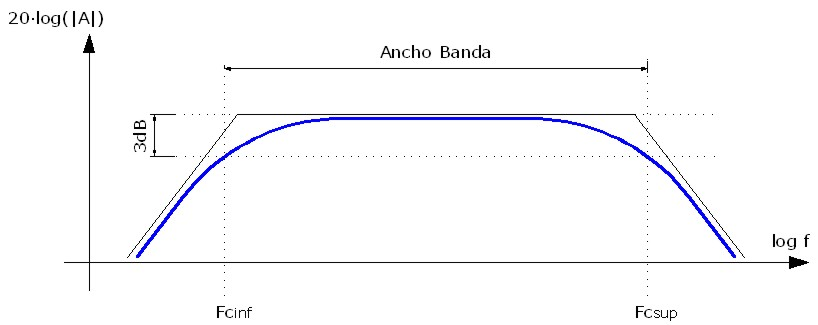
\includegraphics[width=0.9\linewidth]{Imagenes/AnchoBanda.jpg}
    \caption{Ancho de Banda y Frecuencias de Corte}
    \label{fig:AB}
\end{figure}

Una ganancia de -3 dB de su valor original, representa aproximadamente una ganancia del 70,8$\%$ del valor inicial. El cálculo se hace mediante la siguiente fórmula (ecuación \ref{eq:dBaveces}):

\begin{equation}
    \mathrm{dB} = 20 \cdot log \cfrac{G}{G_Q}
    \hspace{0.5cm}\Longrightarrow\hspace{0.5cm}
    G = G_Q \cdot 10^{\frac{\mathrm{dB}}{20}}
    \label{eq:dBaveces}
\end{equation}

Entonces, suponiendo una ganancia inicial en la frecuencia de trabajo de $G_Q$ = 100 (para hacerlo directamente porcentual, o sea que el resultado quede expresado en porcentaje), cuando la ganancia disminuya $3\mathrm{dB}$, se tendrá que la ganancia final será:

\begin{equation}
    -3 \mathrm{dB} = 20 \cdot log \cfrac{G}{100}
    \hspace{0.5cm}\Longrightarrow\hspace{0.5cm}
    G = 100 \cdot 10^{\frac{-3 \mathrm{dB}}{20}} = 70,795
    \label{eq:Gfinal}
\end{equation}

Traduciendo las ganancias a tensiones, se considerará como frecuencias de corte superior e inferior a aquellas frecuencias donde la tensión de salida represente un 70,79$\%$ del valor de tensión típico en la frecuencia de trabajo.

Existen varias maneras de determinar el ancho de banda de un amplificador, pero a lo largo de este trabajo práctico se trabajará principalmente con dos: por barrido en frecuencia y mediante el tiempo de crecimiento ($t_c$).

\subsubsection{Barrido en Frecuencia}

Este es el método más directo de los dos, y como su nombre indica, se realizará un barrido, variando la frecuencia hacia arriba y hacia abajo hasta obtener una tensión de salida de $-3\mathrm{dB}$, partiendo de la frecuencia normal de operación.

Cuando se vea que la tensión de salida llegue al valor calculado, se tomará nota de la frecuencia en la que llegó y luego mediante la ecuación \ref{eq:ABresta}, se obtendrá el ancho de banda.

Este método además de efectivo, si se toman un par de valores intermedios permite graficar fácilmente la forma de la respuesta en frecuencia del amplificador testeado.


\subsubsection{Mediante el tiempo de crecimiento}
\label{sec:AB_tc}

La segunda forma de calcular el Ancho de Banda de la respuesta en frecuencia de un amplificador, es mediante el tiempo de crecimiento $t_c$. Para esto, se conecta la entrada del amplificador a un generador, el cual producirá una onda cuadrada a la frecuencia de trabajo. Las señales de entrada y salida del amplificador se verían de la siguiente manera (figura \ref{fig:slewrate}):

\begin{figure}[H]
    \centering
    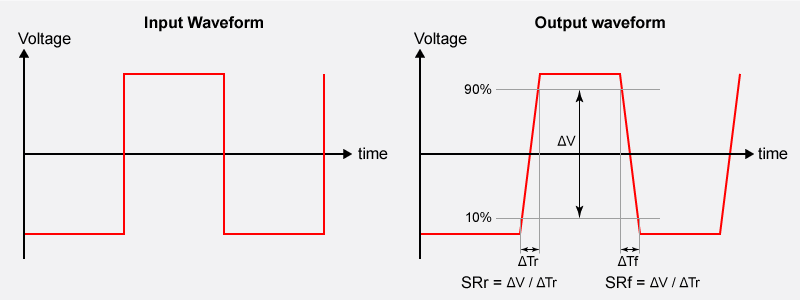
\includegraphics[width=\linewidth]{Imagenes/slewrate.png}
    \caption{Señal de Entrada y de Salida, y tiempos de subida y bajada}
    \label{fig:slewrate}
\end{figure}

En este método, como su nombre lo indica, nos concentraremos en el tiempo de crecimiento $t_c$ de la señal de salida, indicado en la figura \ref{fig:slewrate} como $\Delta Tr$ (de rise time, tiempo de subida en inglés), el cual es el tiempo que toma el amplificador en llevar la tensión de salida del 10$\%$ al 90$\%$ de su valor máximo. Idealmente este tiempo debería ser 0, y la onda de salida debería tener la misma forma que la de entrada, pero en la realidad no es así, existe un retardo de subida y de bajada. Este retardo finalmente será el que limite la frecuencia máxima a la que puede trabajar el amplificador, ya que si la frecuencia supera el tiempo de retardo, el dispositivo no podrá procesar la señal como corresponde.

A partir de la medición de este tiempo de subida, se realizará el cálculo a partir de la siguiente fórmula (ecuación \ref{eq:ABtc}):

\begin{equation}
    t_c = \cfrac{k}{AB}
    \hspace{0.5cm}\Longrightarrow\hspace{0.5cm}
    AB = \frac{k}{t_c}
    \label{eq:ABtc}
\end{equation}

Cabe destacar, que estas ecuaciones son válidas para amplificadores cuya frecuencia de corte inferior es cero o está muy cerca de cero. 

El valor de la constante "k" dependerá de la forma de la caída de la curva de respuesta en frecuencia (Rolloff) en la zona de altas frecuencias.

\begin{figure}[H]
    \centering
    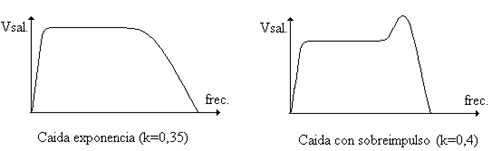
\includegraphics[width=0.87\linewidth]{Imagenes/constK.png}
    \caption{Posibles respuestas del sistema con su \textit{k} correspondiente}
    \label{fig:constk}
\end{figure}

Para conocer el tipo de respuesta del sistema y el \textit{k} a utilizar, se puede realizar un barrido de frecuencias rápido con el generador de funciones y verificar si existe el sobre impulso.

Otra forma, es aplicando una onda cuadrada cuya frecuencia este próxima a la de corte superior del amplificador. Si el borde de subida de la forma de onda obtenida es redondeado, la caída de respuesta es exponencial; en cambio, si el borde presenta picos u oscilaciones, es porque la caída de respuesta es con sobre impulso.

Otra cosa a tener en cuenta, en este método de obtención del Ancho de Banda, es si el tiempo de crecimiento de la onda es muy similar o al menos comparable con el tiempo de crecimiento del osciloscopio. Si es así, se debe aplicar una corrección al valor de $t_c$ del amplificador. 

Como el $t_{c_{osc}}$ depende del ancho de banda del osciloscopio, mediante las siguientes ecuaciones derivadas de la ecuación \ref{eq:ABtc}, se puede obtener su valor:

\begin{equation}
    t_{c_{osc}} = \cfrac{0.35}{AB_{osc}}
    \label{eq:tc_osc}
\end{equation}

Con este valor, se calcula el valor real corregido, del tiempo de subida del amplificador (ecuación \ref{eq:correc}).

\begin{equation}
    t_{c_{amp_{corr}}} = \sqrt{[t_c]^2 + [t_{c_{osc}}]^2}
    \label{eq:correc}
\end{equation}

Ahora si, finalmente se está en condiciones de calcular el ancho de banda, con una mayor exactitud, para lo cual se debe aplicar la fórmula \ref{eq:ABtc}.


%\vspace{1.5cm}
\newpage
\subsection{Máxima Transferencia de Potencia de un Amplificador}
\label{sec:MaxPot}

La potencia máxima que puede entregar un amplificador, se calcula/mide teniendo como carga una resistencia de igual valor que la parte real de la impedancia de salida $Z_o$ del amplificador, debido al \textit{Teorema de Transferencia de Potencia Máxima}, estudiado en la materia \textit{Teoría de Circuitos I}, el cual explica que para cargas resistivas puras, la máxima transferencia de potencia se dará cuando la resistencia de carga sea igual al módulo de la impedancia de salida del circuito al que esta conectada (ecuación \ref{eq:cargaPmax}).

\begin{equation}
    R_{carga} = |Z_o| 
    \label{eq:cargaPmax}
\end{equation}

Como en este trabajo práctico la frecuencia con la que se trabajará es de 1 kHz (baja frecuencia), se consideró la impedancia de salida de ambos amplificadores es totalmente resistiva, por lo que el módulo de esta, será igual a la parte real (resistiva), desembocando en que la resistencia de carga deberá ser igual o lo más parecida posible a ese valor.

